\documentclass{article}
\usepackage[margin=.5in]{geometry}
\usepackage{graphicx, dblfloatfix}
\usepackage{amsmath, amssymb, amsfonts, mathrsfs, mathtools, physics}
\usepackage[english]{babel}
\usepackage[autostyle, english = american]{csquotes}
\usepackage[normalem]{ulem}
\usepackage[title,titletoc,toc]{appendix}
\usepackage{pgfplotstable}
\usepackage{array, booktabs, colortbl, caption}
\MakeOuterQuote{"}

\newcommand{\redchi}{$\tilde{\chi}^2\,$}
\renewcommand{\vec}[1]{\mathbf{#1}}

\title{Compton Scattering}
\author{Alejandro Legarda}

\begin{document}
\raggedright
\maketitle

\begin{abstract}
	We investigate the phenomenon of Compton scattering, and we show how the energy of scattered photons depends on the angle of the scattering. Specifically, we test the validity of the Compton equation for Cs-137 and using an aluminum scatterer.
\end{abstract}
	
	
\tableofcontents
\newpage

\section{Introduction}

For a photon, energy is dependent on momentum in the DeBroglie relation,
\begin{equation*}
	E = \frac{h}{p} = \frac{hc}{\lambda}.
\end{equation*}

When the photon is scattered by an aluminum atom's electron, both energy and momentum must be conserved. Therefore, in order for momentum to be conserved, there must be an energy dependence on angle.

\hspace{.25cm}

Let $\lambda_1$ be the wavelength of the photon before the interaction with the aluminum, and let $\lambda_2$ be the wavelength of the photon after. The momenta are then $p_1$ and $p_2$.

\begin{gather}
	p_1 = \dfrac{h}{\lambda_1}\\
	p_2 = \dfrac{h}{\lambda_2}\\
\end{gather}

By conservation of momentum, and defining $p_\epsilon$ as the difference between the momenta,

\begin{gather}
	\vec{p_1} = \vec{p_2}+\vec{p_{\epsilon}}\\
	p_{\epsilon}^2 = p_1^2 + p_2^2 - 2\vec{p_1} \cdot \vec{p_2}\\
	p_{\epsilon}^2 = p_1^2 + p_2^2 - 2p_1p_2\cos\theta
\end{gather}

Conservation of energy gives

\begin{gather}
	p_1 c + E_0 = p_2 c + \sqrt{E_0^2 + p_{\epsilon}^2}\\
	p_1^2 c^2 + E_0^2  + 2p_1 c E_0= p_2^2 c^2 + E_0^2 + p_{\epsilon}^2\\
	p_{\epsilon}^2 = p_1^2 + p_2^2 - 2p_1p_2 + \frac{2E_0(p_1 - p_2)}{c}
\end{gather}

Equating the two expressions for $p_{\epsilon}^2$ yields

\begin{gather}
	\frac{E_0 (p_1 - p_2)}{c} = p_1 p_2 (1 - \cos \theta)\\
	\lambda_2 - \lambda_1 = \frac{hc}{E_0} (1 - \cos \theta)
\end{gather}

Knowing $E_{Compton} = \frac{hc}{\lambda_2}$ we obtain

\begin{equation}
	E_{Compton} = \dfrac{E_0}{1+\dfrac{E_0}{mc^{2}}(1-\cos \theta)}.
\end{equation}

\section{Method}
\subsection{Apparatus}


\begin{figure}[!htb]
	\centering
	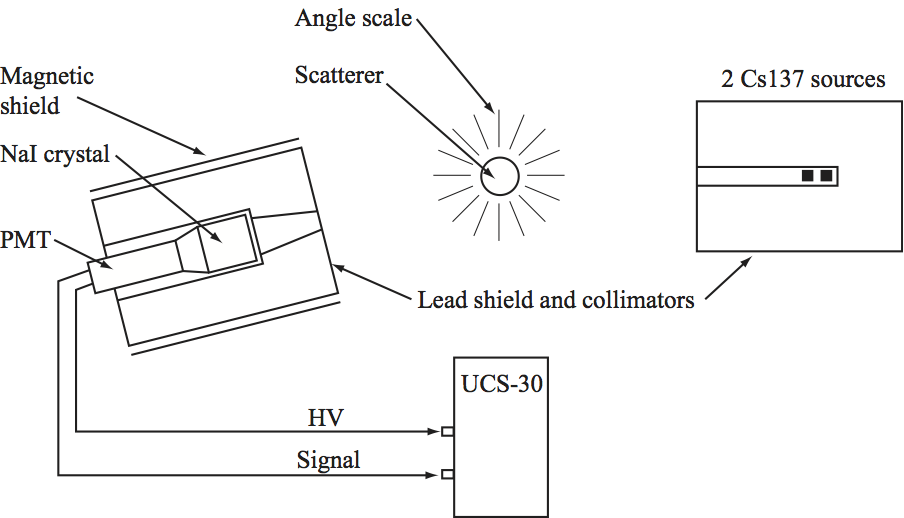
\includegraphics[scale=.8]{plots/Compton_apparatus.png}
  	\caption{The experimental setup.} 
 	\label{Apparatus}
\end{figure}

Our setup consists of a pair of radioactive Caesium-137 sources housed in a radio-insulating box with a narrow opening. These produce gamma rays at 662 keV, which come out the opening as a collimated beam. The radioactive decay is directed at a cylindrical aluminum rod that scatters incoming photons at random angles – some energy loss is incurred. Finally, we have a NaI crystal and behind it a photomultiplier tube housed, again, in a radio-insulating box with a narrow opening that points at the scatterer. Each photon that strikes the NaI crystal will produce an output from the PMT. The size of the PMT pulses will be proportional to the energy of the photons that caused them. This signal is then sent to a PHA for quantification, and the data is then finally stored as a histogram on the computer. The PMT is mounted on a rail such that we can alter the angle between the PMT and the original sources without changing the distance from the PMT to the scatterer.

\hspace{.25cm}

For this lab, we use a crystal of sodium iodide doped with thallium as our detector. Iodine is a high Z material, so there is a large cross section for interaction for photons passing through the detector. When a high-energy photon scatters in the crystal, electrons carry away the deposited energy and are propelled through the solid. These high energy electrons knock into other electrons and create many smaller energy events, known as an electron shower. In turn, the thallium dopant is excited, and when it quickly de-excites, new photons are emitted. The amount of light given off by the thallium dopant is proportional to the energy left by the initial higher-energy photon. This process is called scintillation. Impurities will mean less light given out in proportion to energy, or even disruption of the linear relationship.

In order to make use of this new scintillation light, the crystal is optically coupled to a photomultiplier tube (PMT). This tube is a series of dynodes each held at a higher voltage potential. The scintillation photons released by the thallium are absorbed in the first dynode of the PMT and kick out electrons via the photoelectric effect. These electrons are accelerated toward the next dynode where they produce more electrons.  At each stage the number of electrons kicked out exceeds the number of electrons coming in, so a small input signal gets "multiplied" into a larger output signal at the final plate. The multiplication factor of the PMT is determined by the number of dynodes and the applied high voltage.

\subsection{Energy Calibration}
As mentioned earlier, the data from the PMT is stored as a histogram. However, our x-axis will need calibration, as the PHA will only know to assign higher energies to higher channel numbers. We do not calibrate directly on the PHA software, as we expect some drift to the (true) calibration throughout the experimental procedure. We use a 3-point calibration using the known energies of Ba-133 and Cs-137 gamma decay peaks. We chose Ba-133 because it conveniently gives us two peaks, so we can very confidently place two calibration points at the same time. We use the formula from our introduction for the Compton energy, and we use the maximum angle of 135 degrees to obtain real energy values to assign to the centroids of our peaks on the computer software. This allows us to convert channel number to energy in keV. We have two sets of calibration data, one for each day of the experiment:

\begin{center}
    \centering
    \captionof{table}{Day 1 Calibration - Start} \label{tab:title} 
    \begin{tabular}{| l | l | l |}
    \hline
    Source & Channel Number & Energy [keV] \\ \hline
    Ba-133 & 118 $\pm 3$ & 81 \\ \hline
    Ba-133 & 505 $\pm 3$ & 356 \\ \hline
    Cs-137 & 921 $\pm 3$ & 662 \\ \hline
    \end{tabular}
\end{center}

Due to our equipment shutting off at the end of day 1, we decided that it would not be beneficial to take a second set of calibration measurements. We assume a linear relationship between channel number and energy, and produce the following fit.

\begin{figure}[!htb]
	\centering
	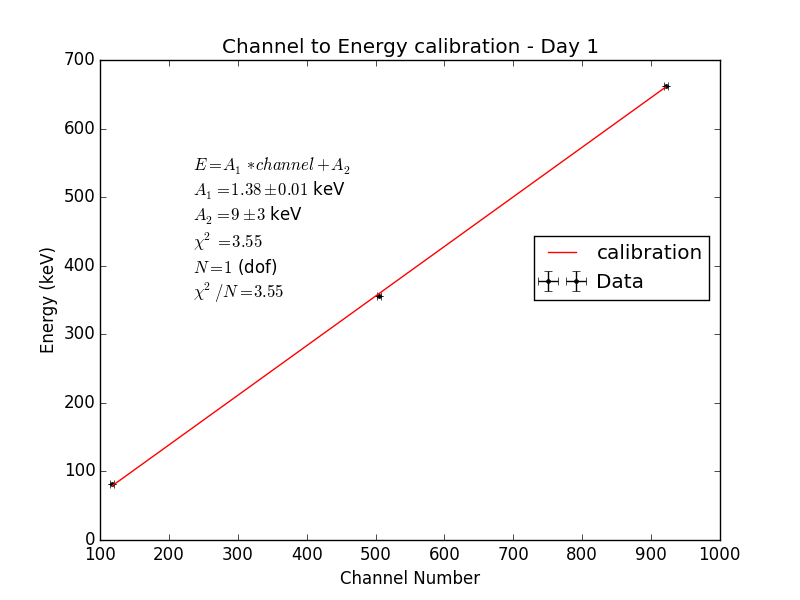
\includegraphics[scale=.75]{plots/cal1.png}
  	\caption{Calibration for Day 1.} 
 	\label{cal1}
\end{figure}

\begin{center}
    \centering
    \captionof{table}{Day 2 Calibration - Start} \label{tab:title} 
    \begin{tabular}{| l | l | l |}
    \hline
    Source & Channel Number & Energy [keV] \\ \hline
    Ba-133 & 117 $\pm 3$ & 81 \\ \hline
    Ba-133 & 499 $\pm 3$ & 356 \\ \hline
    Cs-137 & 909 $\pm 3$ & 662 \\ \hline
    \end{tabular}
\end{center}

\begin{center}
    \centering
    \captionof{table}{Day 2 Calibration - End} \label{tab:title} 
    \begin{tabular}{| l | l | l |}
    \hline
    Source & Channel Number & Energy [keV] \\ \hline
    Ba-133 & 116 $\pm 3$ & 81 \\ \hline
    Ba-133 & 498 $\pm 3$ & 356 \\ \hline
    Cs-137 & 903 $\pm 3$ & 662 \\ \hline
    \end{tabular}
\end{center}

For day 2, however, we will use an average of our calibration data to do the actual calibration, in an effort to minimize error due to drift.

\begin{figure}[!htb]
	\centering
	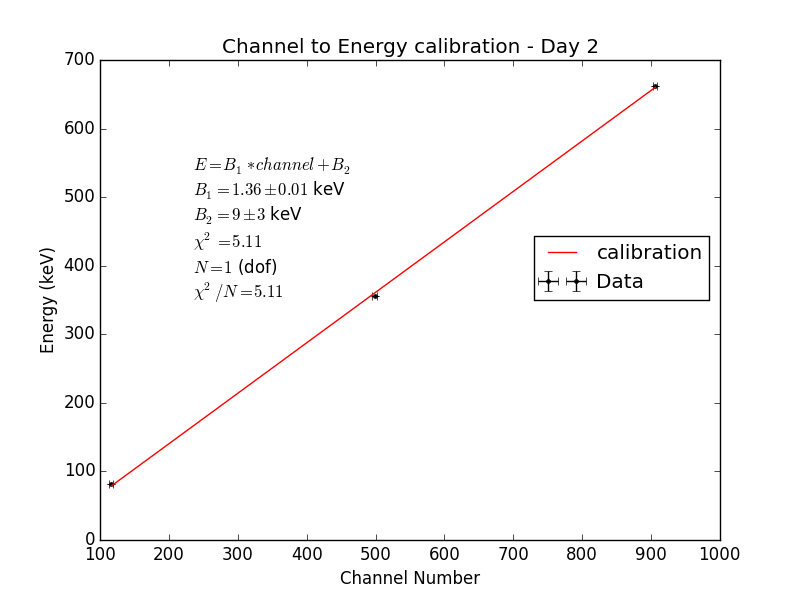
\includegraphics[scale=.75]{plots/cal2.png}
  	\caption{Calibration for Day 2.} 
 	\label{cal2}
\end{figure}

\hspace{.25cm}

We are now able to convert any measured channels directly into energy in keV, with some error that we calculate from the error in the fit parameters. The primary source of error in the calibration is the measurement of the centroid of the peak on the PHA. We assume an error of $\pm 3$ for our centroid measurements, which is due to visual restrictions and the fact that centroid is given as an integer. The conversion from channel number to energy in keV is roughly given by

\begin{equation}
	E = 1.37 * channel + 9 .
\end{equation}


\section{Analysis}
\subsection{Scattering Relation}

Using our calibration from before, we can now plot energy against angle to test the Compton relation. We fit the form of equation (12) to our data, leaving the energy of the initial gamma rays and the rest mass-energy of the electron as free parameters for the fit to determine.

\begin{figure}[!htb]
	\centering
	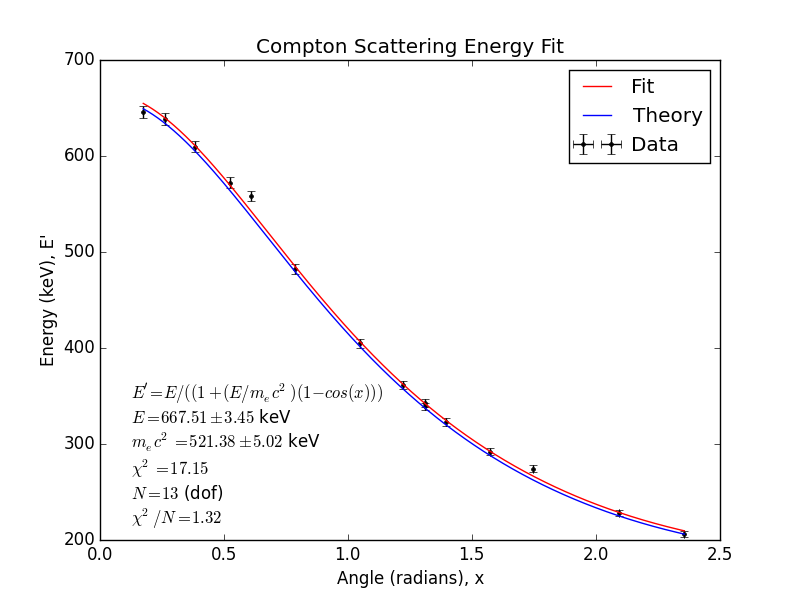
\includegraphics[scale=1]{plots/compton_fit.png}
  	\caption{Compton Scattering Relation.} 
 	\label{compton}
\end{figure}

This gives us a rest mass for the electron of

\begin{equation}
	m_e = \frac{521.38}{c^2} = 0.521 \pm 0.005 MeV/c^2 
\end{equation}

This is close to, but does not overlap with the literature value of $m_e = 0.511 MeV/c^2$.

\subsection{Uncertainties}
It is worth discussing our sources of uncertainty for our data and this fit. One of the biggest sources of uncertainty is, as discussed earlier, the measurement of the centroid of the peaks. This introduces the most significant error in energy measurements. Angle measurement errors, although not accounted for in our fitting, provides the most significant source of error in our x-axis. Furthermore, there seems to be, upon comparing our fitted line and the literature line, some systematic error in energy measurements: our fitting function appears to be shifted down by a mostly constant amount compared to the literature line. This can explain the discrepancy between our measurement for the electron rest mass and the literature's.

\hspace{.25cm}

Uncertainties in the calibration, which where overwhelmingly from centroid measurement, were propagated into the function that converts channel into energy. By first fitting for channel as a function of energy, we were able to use our uncertainties as errors in y, making the fitting process easier. We then simply propagated the error in the parameters of channel as a function of energy into the parameters for the inverse of this function. Now, having translate uncertainties in x into uncertainties in y (energy), we can properly account for statistical and measurement errors on an energy vs angle plot.

\section{Conclusion}

We conclude that our data and fits show the Compton relation well. The form of the fitted and literature functions both fit the data reasonably well, so we can be confident on the form of the relationship. Our biggest issue seems to be the systematic lower-than-actual energy measurements, as can be seen in our final plot. This could be simply due to energy loss somewhere in the apparatus before the quantification of photon energy is done.
Overall, our data agrees well with the expected relationship from the Compton scattering formula, but is not useful for extracting fine constants such as the electron rest mass.


\begin{thebibliography}{10}

	\bibitem{lab manual}
		University of Chicago Department of Physics. "Compton Scattering"\\
		https://wiki.uchicago.edu/display/P211manuals/Compton+Scattering. (Accessed Feb, 2016)

	\bibitem{taylor}
		Taylor, John. \emph{An Introduction to Error Analysis}. Sausalito: University Science Books, 1997.
		
\end{thebibliography}

\end{document}